\section{Fuzzy mathematics}

Fuzzy numbers are a mathematical concept used to model our perception of approximate values. 
They are essentially fuzzy sets defined over the set of real numbers. 
Three important constraints are used to define fuzzy numbers:
\begin{enumerate}
    \item Normal fuzzy sets: fuzzy numbers adhere to the principles of normal fuzzy sets, which allows them to capture the concept of approximate value.
    \item Convex fuzzy sets: for a fuzzy number to be well-defined, all $\alpha$-cut intervals should be closed. This is a key constraint for arithmetic operations.
    \item Bounded support: the support of a fuzzy number (the range where it has significant membership) should be bounded, providing further constraints for their definition.
\end{enumerate}
Fuzzy sets can be used to define various types of numerical representations, including fuzzy numbers, fuzzy intervals, defined intervals, and crisp numbers, as illustrated in the provided figure.
\begin{figure}[H]
    \centering
    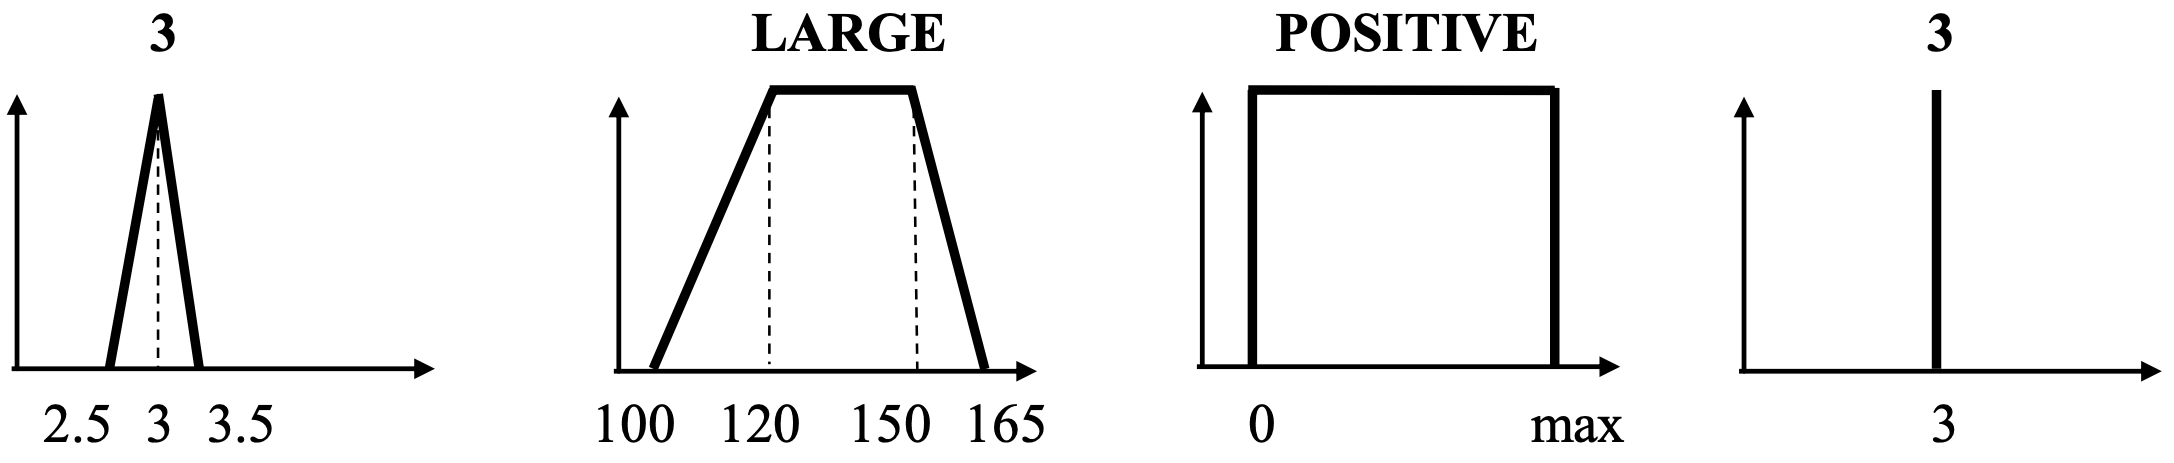
\includegraphics[width=0.75\linewidth]{images/numbers.png}
    \caption{Possible representation of numbers}.
\end{figure}
The arithmetic of fuzzy numbers is based on two primary properties:
\begin{itemize}
    \item Uniqueness of $\alpha$-cuts: each fuzzy number can be fully represented by its $\alpha$-cuts, which are unique for that number.
    \item Closed intervals: the $\alpha$-cuts of fuzzy numbers are closed intervals of real numbers, which is crucial for arithmetic operations.
\end{itemize}
The four main arithmetic operators for fuzzy numbers are defined by combining operations on the intervals (represented by $\alpha$-cuts) that make up the fuzzy number:
\begin{itemize}
    \item Addition: $[a,b]+[d,e]=[a+d,b+e]$.
    \item Subtraction: $[a,b]-[d,e]=[a-e,b-d]$.
    \item Multiplication:  $[a,b] \times [d,e]=[\min (ad,ae,bd,be),\max (ad,ae,bd,be)]$
    \item Division: $[a,b] \div [d,e]=\left[\min \left(\dfrac{a}{d},\dfrac{a}{e},\dfrac{b}{d},\dfrac{b}{e}\right),\max \left(\dfrac{a}{d},\dfrac{a}{e},\dfrac{b}{d},\dfrac{b}{e}\right)\right]$ with the condition that $[d,e] \neq [0,0]$ to avoid division by zero.
\end{itemize}
These operators allow for performing arithmetic operations on fuzzy numbers, taking into account the uncertainty or fuzziness associated with each value.
\begin{example}
    Given the fuzzy numbers $[1,3]$ and $[4,6]$, we have the following operations:
    \begin{itemize}
        \item Addition of fuzzy numbers: the sum is calculated as the sum of the minimum and maximum values in each interval, resulting in 
        \[[1,3] + [4,6] = [1+4, 3+6] = [5,9]\]
        Graphically, this operation is represented as follows:
            \begin{figure}[H]
                \centering
                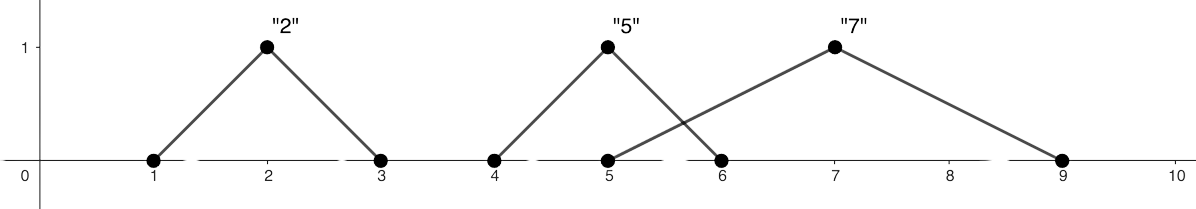
\includegraphics[width=0.75\linewidth]{images/sum.png}
            \end{figure}
        \item Subtraction of fuzzy numbers: the difference is found by subtracting the minimum of the first interval from the maximum of the second and subtracting the maximum of the first interval from the minimum of the second, yielding 
        \[[1,3] - [4,6] = [1-6, 3-4] = [-5,-1]\]
        Graphically, this operation is shown below:
            \begin{figure}[H]
                \centering
                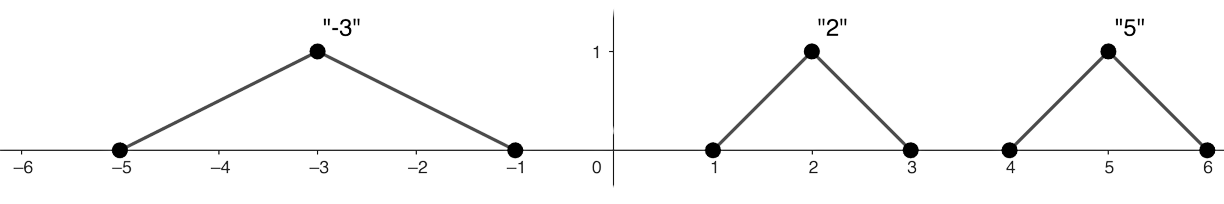
\includegraphics[width=0.75\linewidth]{images/subtraction.png}
            \end{figure}
        \item Multiplication of fuzzy numbers: the product is determined by taking the minimum and maximum values of the products of corresponding elements, resulting in 
        \[[1,3] \times [4,6] = [\min(1 \cdot 4, 1 \cdot 6, 3 \cdot 4, 3 \cdot 6), \max(1 \cdot 4, 1 \cdot 6, 3 \cdot 4, 3 \cdot 6)] = [4,18]\]
        Graphically, this operation is represented as follows:
            \begin{figure}[H]
                \centering
                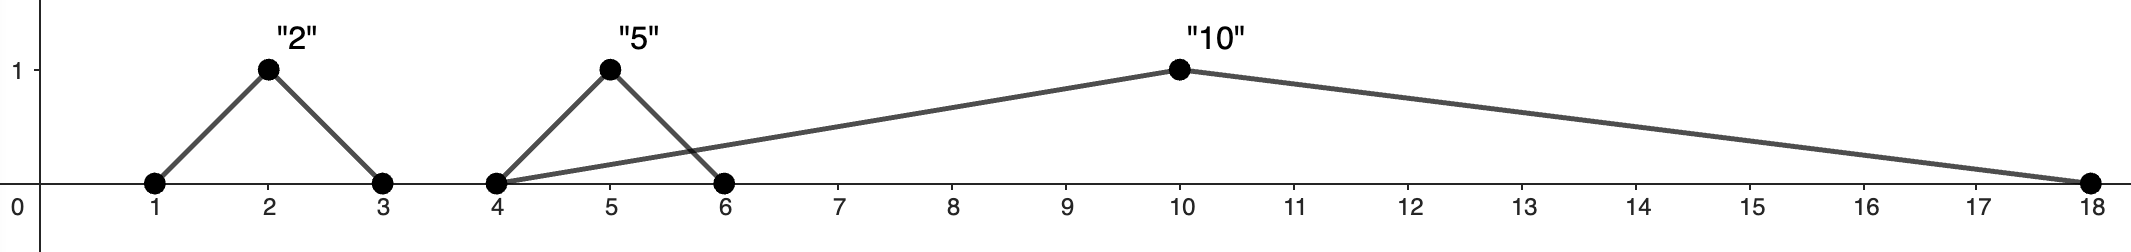
\includegraphics[width=0.75\linewidth]{images/multiplication.png}
            \end{figure}
        \item Division of fuzzy numbers: the division is obtained by finding the minimum and maximum values of the divisions of corresponding elements, leading to:
        \[[1,3] \times [4,6]=\left[\min\left(\dfrac{1}{4}, \dfrac{1}{6}, \dfrac{3}{4}, \dfrac{3}{6}\right),\max\left(\dfrac{1}{4}, \dfrac{1}{6}, \dfrac{3}{4}, \dfrac{3}{6}\right)\right]=\left[\dfrac{1}{6},\dfrac{3}{4}\right]\]
        Graphically, this operation is shown as follows:
            \begin{figure}[H]
                \centering
                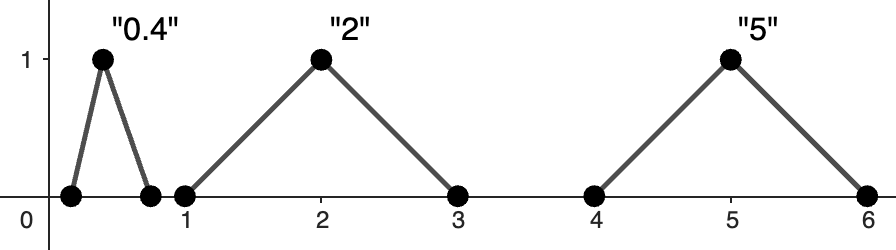
\includegraphics[width=0.5\linewidth]{images/division.png}
            \end{figure}
    \end{itemize}
\end{example}
From fuzzy arithmetic, it is also possible to define fuzzy functions, fuzzy integrals, and fuzzy derivatives. 
In general, fuzzy numbers are employed to represent approximations.